\documentclass{article}
\usepackage[top=0.1in, bottom=0.5in, left=0.5in, right=0.5in]{geometry}

\begin{document}
\section{Introduction}
We began our journey with word vectors. We looked at vectors on 2D plane in using python to understand analogies and importance of word vectors. Then we moved to RNNS (Recurrent Neural Networks). This architecture had vanishing gradients problem (gradients diminish exponentially as they are propagated back through time) which prevented it from learning long-term dependences in sequences. This issue was partially resolved by LSTMS (Long Short-Term Memory). We used LSTMs for neural machine translation. This was an interesting task. However, it was slow due to its sequential processing of input embeddings. We then moved to transformers to utilize the parallel processing capabilities of GPUs.
\subsection{Recurrent Neural Networks(RNNs)}
Let's first talk a briefly about RNNs. RNNs are a class of Neural Networks which take inputs sequentially and produce a hidden state.

\begin{figure}[ht!]
\centering
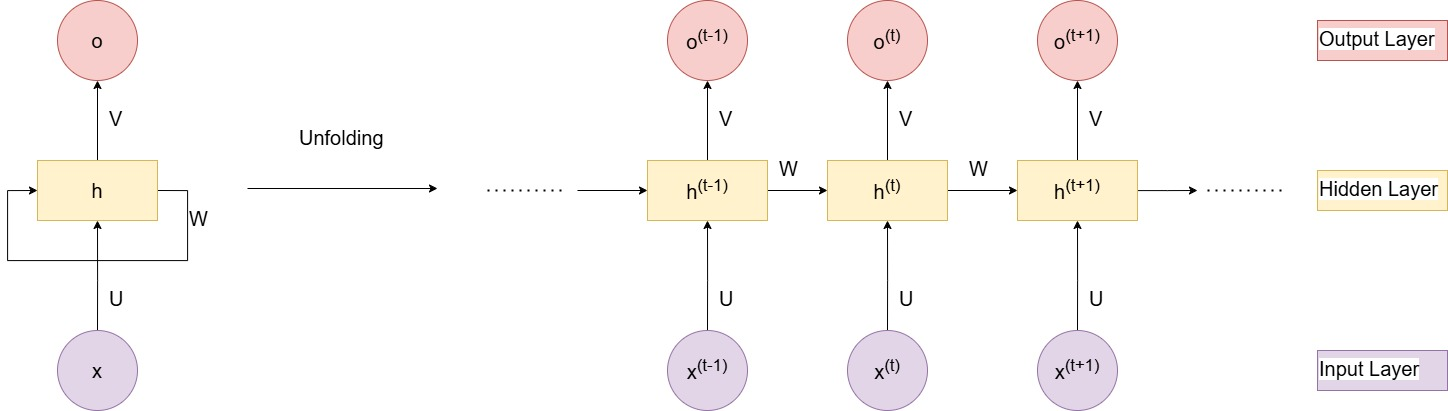
\includegraphics[width=90mm]{Images/RNN.jpg}
\caption{Basic RNN structure. Here x is input sequence, o is output sequence, and h is the hidden state. U, V, and W are training weights\label{overflow}}
\end{figure}

The hidden state is calculated using the following equation:
\begin{equation} \label{eqn1}
h_t = {g(Uh_{t-1}+Wx_{t-1})}
\end{equation}
Here, \(h_t\) is the hidden state at time t, g is the activation function.

Then, using the following equation output is calculated:
\begin{equation} \label{eqn2}
o_t = {f(Vh_t)}
\end{equation}
Here, \(o_t\) is the output at time t, f is another activation function.

We studied bidirectional RNNs. \textbf{Biderection RNN} combines two independent RNNs, one where the input is processed from the start to the end and the other where the input is processed from the end to the start. We then concatenate the two hidden states into one vector. This vector captures both left and right contexts of an input at each point in time. Vector concatenation is shown like this:
\begin{equation} \label{eqn3}
h_t={[h_t^f;h_t^b]}
\end{equation}
RNNs are good at learning short term dependencies but fail to learn short term dependencies becauuse of the vanishing graddients problem.

\subsection{Long Short-Term Memory (LSTM)}
Long Short-Term Memory (LSTM) networks are an advanced type of recurrent
neural network (RNN) designed to handle sequential data while addressing the
vanishing gradient problem to some extent. LSTMs achieve this by introducing
memory cells and gating mechanisms that regulate the flow of information.

An LSTM cell consists of three primary gates:
\begin{itemize}
    \item \textbf{Forget Gate}: Determines which part of the previous cell state (C\_{t-1})
    should be discarded:
    \begin{equation} \label{eqn4}
        \text{f}_t = {\sigma}(\text{W}_f\cdot[\text{h}_{t-1},\text{x}_t] + \text{b}_f)
    \end{equation}
    where \(\text{f}_t\) is the forget gate output, \(\text{W}_f\) and \(\text{b}_f\) are the weights and biases, \(\text{h}_{t-1}\) is the hidden state from the previous time step, and xt is the current input.
    \item \textbf{Input Gate}: Decides which new information to store in the cell state:
    \begin{equation} \label{eqn5}
        \text{i}_t = {\sigma}(\text{W}_i\cdot[\text{h}_{t-1},\text{x}_t] + \text{b}_i)
    \end{equation}
    \begin{equation} \label{eqn6}
        \tilde{\text{c}}_t = {\tanh}(\text{W}_c\cdot[\text{h}_{t-1},\text{x}_t] + \text{b}_c)
    \end{equation}
    Here, it is the input gate output, and $\tilde{\text{c}}_t$ is the candidate cell state.
    \item \textbf{Cell State Update}: Combines the forget and input gates to update the
    cell state:
    \begin{equation} \label{eqn7}
        \text{i}_t = (\text{f}_t \cdot \text{C}_{t-1} + \text{i}_t \cdot \tilde{\text{C}}_t)
    \end{equation}
    \item \textbf{Output Gate}: Produces the new hidden state (ht):
    \begin{equation} \label{eqn8}
        \text{o}_t = {\sigma}(\text{W}_o\cdot[\text{h}_{t-1},\text{x}_t] + \text{b}_o)
    \end{equation}
    \begin{equation} \label{eqn9}
        \text{h}_t = \text{o}_t\cdot \tanh(\text{C}_t)
    \end{equation}
\end{itemize}
In the equations above, $\sigma$ is the sigmoid activation function, and tanh is the hyperbolic tangent function. LSTMs use these mechanisms to store, update, and retrieve information effectively, making them suitable for tasks like time series prediction, natural language processing, and speech recognition.
% \write18{wget https://www.researchgate.net/profile/Savvas-Varsamopoulos/publication/329362532/figure/fig5/AS:699592479870977@1543807253596/Structure-of-the-LSTM-cell-and-equations-that-describe-the-gates-of-an-LSTM-cell.jpg}
% \includegraphics{image.jpg}

\subsection{Transformers}
Transformer, as described in the paper “Attention is all you need” and introduced in 2017 is an architecture that transforms one sequence into another sequence by using two blocks: Encoder and Decoder. Unlike LSTMs, RNNs etc. which used sequence-to-sequence techniques to process the data, transformer processes the data in parallel and relies on attention mechanisms, thus improving efficiency and performance. The advantage of attention mechanisms is that it speeds up the translation processed by the model. Some of the key components of the Transformer are as follows:
\subsubsection{}
\subsection{Bidirectional Encoder Representations from Transformers: BERT}
\subsubsection{Introduction}
Prior to BERT word embedding models like Word2Vec1 and GloVe2 provide static representations 
for words where the same word like “bank” would always map on same vector. It doesn't depends 
on the context in which it is used. They were effective for some task but struggled with contextual 
meaning of sentence. The advent of transformer architecture with it's self-attention mechanism 
firstly enabled parallel processing solving a major problem of not utilising complete power of GPUs 
but also enabled long range dependency modeling. BERT was introduced in 2018 which leveraged 
these advancements to create deeply bidirectional contextual embedding revolutionizing Natural 
Language Processing (NLP).
\subsubsection{Architecture}
BERT's architecture is based on transformer encode from Vasani et al. 3, which uses stacked slef
attention layers to process input sequence in parallel. Unlike decoder based models BERT uses the 
encoder to generate representation bidirectionally. Key architectural features includes Multi head 
self-attention, Positional embedding, Layer normalization and Residual connections that helps 
captures contextual relationship with words injects position of each word into the input tokens and 
stabilizes the training in deep networks respectively. BERT has two primary configurations:
 BERT-base (12 layers, 786 hidden dimensions, 12 attention heads)
 BERT-large(24 layers, 1024 hidden dimensions, 16 attention heads)
\paragraph{Tokenization}
\section{Tasks}
\subsection{Week 1}
\subsubsection{Rooshan Khan: Attention Method in bert.py}
